

% \section{Изучение материала}
% В ходе выполнения преддипломной практики были изучены следующие источники, в которых описывались методы прогнозирования интервальных данных:
% \begin{enumerate}
%     \item \label{en1}Linear regression analysis for interval-valued data based on the Lasso technique \cite{interval_valued};
%     \item \label{en2}Interval linear regression methods based on minkowski difference. \cite{minkowski}
% \end{enumerate}

% В источнике \ref{en2} предлагаются методы линейной регрессии, основанные на метрике Минковского.

% В источнике \ref{en1} для каждого $x_{ij}$ имеется середина  и радиус интервала, в котором он лежит. Соответственно, каждый $y_i$ определяется серединой некоторого интервала и его радиусом.
% То есть:
% \begin{eqnarray}
%     y_{i_M} = b_{M_0} + b_{M_1} x_{M_{i1}} + \dots + b_{M_n} x_{M_{in}} + \varepsilon_{M_i}\\
%     y_{i_R} = b_{R_0} + b_{R_1} x_{R_{i1}} + \dots + b_{R_n} x_{R_{in}} + \varepsilon_{R_i}
% \end{eqnarray} 
% Решается задача:
% \begin{eqnarray}
%     \min_{b_{M_0},\dots,b_{M_n},b_{R_0}, \dots, b_{R_n}} \sum\limits_{i=1}^N [(\varepsilon_{M_i})^2 + (\varepsilon_{R_i})^2]
% \end{eqnarray}
\section{Альтернативные оценки параметров модели}
Рассмотрим альтернативный метод оценивания параметров модели регрессии, основанный на замене группированных наблюдений серединами соответствующих интервалов. 
Такой метод встречается в литературе, например в \cite{interval_valued}.

Метод заключается в следующем:
пусть имеется $\mu_i$ - номер полуинтервала, в который попало очередное наблюдение $y_i$. Ему соответствует полуинтервал $\nu_{\mu_i}$ (из (\ref{eq13})), т.е. полуинтервал:
\begin{eqnarray}
    y_i\in (a_{\nu_{\mu_i}},a_{\nu_{\mu_i}+1}], i = \overline{1,N}
\end{eqnarray}
(считаем что $a_1<y_i<a_{k-1}, i=\overline{1,N}$, т.е $1\leq\mu_i\leq k-2$).

Найдем центральную точку этого интервала, т.е. точку
\begin{eqnarray}
    \check{y_i} = \frac{a_{\nu_{\mu_i}} + a_{\nu_{\mu_i}+1}}{2}
\end{eqnarray}

Построим для всех значений функции регрессии $y_i$ значения $\check{y_i}$.
Будем использовать в качестве значений функции регрессии полученные значения $\check{y_i}$, а в качестве регрессоров $x_i$ и построим МНК оценки параметров $\beta$.

\newpage
\section{Полиномиальная регрессия}
Введем теперь модель полиномиальной регрессии.

\begin{equation}
    \begin{array}{c}
        \label{eq28}y_i=\beta_0+\beta_1 x_{i1}^1+\beta_2 x_{i2}^2+\dots+\beta_n x_{in}^n+\varepsilon_i, i=\overline{1,N},\\
        y_i = \sum\limits_{l=1}^{n} x_{il}^{l-1} + \varepsilon_i, i=\overline{1,N},\\
        y_i= f(x_i,\beta)+\varepsilon_i,\\
        f(x_i,\beta)=\beta_0+\beta_1 x_{i1}^1+\beta_2 x_{i2}^2+\dots+\beta_n x_{in}^n
    \end{array}
\end{equation}
В случае полиномиальной регрессии также справедливо:
\begin{eqnarray}
    y_i=f(x_i,\beta)+\varepsilon_i \sim \mathcal{N}(f(x_i,\beta),\sigma^2).
\end{eqnarray}

Поскольку оценки строились путём максимизирования функции:
\begin{eqnarray}
    l(\beta,\sigma^2, \nu_0,\dots, \nu_{k-1})&=&\sum_{i=1}^{n}\ln(P(\mu_i=j))=\\
    &=&\begin{cases}
        \frac{1}{2}(\textup{erf}(\frac{a_{j+1}-f(x_i,\beta)}{\sqrt{2}\sigma})-\textup{erf}(\frac{a_{j}-f(x_i,\beta)}{\sqrt{2}\sigma})),~j=\overline{1,k-2}\\
        \frac{1}{2}(1+\textup{erf}(\frac{a_{1}-f(x_i,\beta)}{\sqrt{2}\sigma})),~j=0\\
        \frac{1}{2}(1+\textup{erf}(\frac{a_{k-1}-f(x_i,\beta)}{\sqrt{2}\sigma})),~j=k-1
    \end{cases},
\end{eqnarray}
а функция правдоподобия максимизировалась путём решения системы уравнений:
\begin{equation}
    \frac{\delta l}{\delta \beta}=0,
\end{equation}
где:
\begin{multline}
    \frac{\delta l}{\delta \beta}=\frac{\delta \sum_{i=1}^{n}\ln(P(\mu_i=j))}{\delta \beta}=\frac{\delta \sum_{i=1}^{n}\ln P(y_i\in \nu_{\mu_i})}{\delta \beta}=~\\
    =\frac{\delta \sum_{i=1}^{n} \ln(\frac{1}{2}(\textup{erf}(\frac{a_{\mu_i+1}-f(x_i,\beta)}{\sqrt{2}\sigma})-\textup{erf}(\frac{a_{\mu_i}-f(x_i,\beta)}{\sqrt{2}\sigma})) )         }{\delta \beta}=~\\
    =  \sum_{i=1}^{n}\Big((1-(\delta_{\mu_i 0}+\delta_{\mu_i k-1}))\frac{(\textup{erf'}(\frac{a_{\mu_i+1}-f(x_i,\beta)}{\sqrt{2}\sigma})-\textup{erf'}(\frac{a_{\mu_i}-f(x_i,\beta)}{\sqrt{2}\sigma}))}{ (\textup{erf}(\frac{a_{\mu_i+1}-f(x_i,\beta)}{\sqrt{2}\sigma})-\textup{erf}(\frac{a_{\mu_i}-f(x_i,\beta)}{\sqrt{2}\sigma}))}+~\\
    +(\delta_{\mu_i 0}+\delta_{\mu_i k-1})\frac{\textup{erf'}(\frac{a_{\mu_i}-f(x_i,\beta)}{\sqrt{2}\sigma})}{(1+\textup{erf}(\frac{a_{\mu_i}-f(x_i,\beta)}{\sqrt{2}\sigma}))}\Big)  (-1) \frac{\delta f(x_i,\beta)}{\delta \beta} )=~
\end{multline}
\begin{multline}
    \nonumber 
    =-\sum_{i=1}^{n}\begin{pmatrix}
        1\\
        x_{i1}\\
        \dots\\
        x_{in}
    \end{pmatrix}\times  \Big((1-(\delta_{\mu_i 0}+\delta_{\mu_i k-1}))\frac{(\textup{erf'}(\frac{a_{\mu_i+1}-f(x_i,\beta)}{\sqrt{2}\sigma})-\textup{erf'}(\frac{a_{\mu_i}-f(x_i,\beta)}{\sqrt{2}\sigma}))}{ (\textup{erf}(\frac{a_{\mu_i+1}-f(x_i,\beta)}{\sqrt{2}\sigma})-\textup{erf}(\frac{a_{\mu_i}-f(x_i,\beta)}{\sqrt{2}\sigma}))}+~\\
    +(\delta_{\mu_i 0}+\delta_{\mu_i k-1})\frac{\textup{erf'}(\frac{a_{\mu_i}-f(x_i,\beta)}{\sqrt{2}\sigma})}{(1+\textup{erf}(\frac{a_{\mu_i}-f(x_i,\beta)}{\sqrt{2}\sigma}))}\Big),
\end{multline}
то построенные оценки также применимы и для полиномиальной регрессии.

Также как и в случае линейной регрессии считаем, что выборка содержит выбросы, т.е., аналогично:
\begin{eqnarray}
    y_i^{\widetilde{\varepsilon}}=(\xi_i)y_i+ (1-\xi_i)\eta_i,
\end{eqnarray}
здесь $y_i$ задаются формулой (\ref{eq28}).

\newpage
\section{Компьютерные эксперименты}
% \subsection{Параметры модели и оценок}
% В ходе экспериментов использовались следующие параметры модели:
% \begin{center}
%     \begin{tabular}{|p{5cm}|p{5cm}|}
%         \hline
%         \multicolumn{2}{|c|}{Параметры программы} \\
%         \hline
%         Переменная&значение\\
%         \hline
%         Размер выборки $N$& 1000\\
%         \hline
%         Доля выбросов $\widetilde{\varepsilon}$& 0.08\\
%         \hline
%         Параметры регрессии $\beta$& $(90,4)$\\
%         \hline
%         Регрессоры $x_i$ & $\sim U(-5,5)$\\
%         \hline
%         $\varepsilon_i$&$\sim N(0,16)$\\
%         \hline
%         $\eta_i$&$\sim N(100,100)$\\
%         \hline
%         Величина $K$ из пункта 2.3 курсового проекта &$10$\\
%         \hline
%     \end{tabular},
% \end{center}
% \newpage

\subsection{Сравнительный анализ построенной оценки с альтернативной}
\subsubsection{Эксперимент с изменением объема выборки}
В следующем эксперименте был произведен сравнительный анализ вариаций ОМП-оценок с МНК оценками в зависимости от объема выборки.

Объем выборки $N$ изменялся от $N_1=100$ до $N_2=500$, при этом выборка дополнялась, а не генерировалась новая. Использовалась модель линейной регрессии. Доля выбросов была постоянна и равнялась $\widetilde{\varepsilon}=0.08$. Параметры регрессии были постоянными и равнялись $\beta=(90,4)^T$. 
Регрессоры $x_i$ были из равномерного распределения $U(-5,5)$, ошибки эспериментов $\varepsilon_i\sim \mathcal{N}(0,16)$.

\begin{center}
    \captionof{table}{Параметры модели и оценок}\label{tab1}
    \begin{tabular}{|p{5cm}|p{5cm}|}
        \hline
        \multicolumn{2}{|c|}{Параметры программы} \\
        \hline
        Переменная&значение\\
        \hline
        Размер выборки $N$& от 100 до 500\\
        \hline
        Доля выбросов $\widetilde{\varepsilon}$& 0.08\\
        \hline
        Параметры регрессии $\beta$& $(90,4)$\\
        \hline
        Регрессоры $x_i$ & $\sim U(-5,5)$\\
        \hline
        $\varepsilon_i$&$\sim \mathcal{N}(0,16)$\\
        \hline
        $\eta_i$&$\sim \mathcal{N}(100,100)$\\
        \hline
        Величина $K$  &$10$\\
        \hline
    \end{tabular},
\end{center}
\begin{figure}[h!]
    \centering
    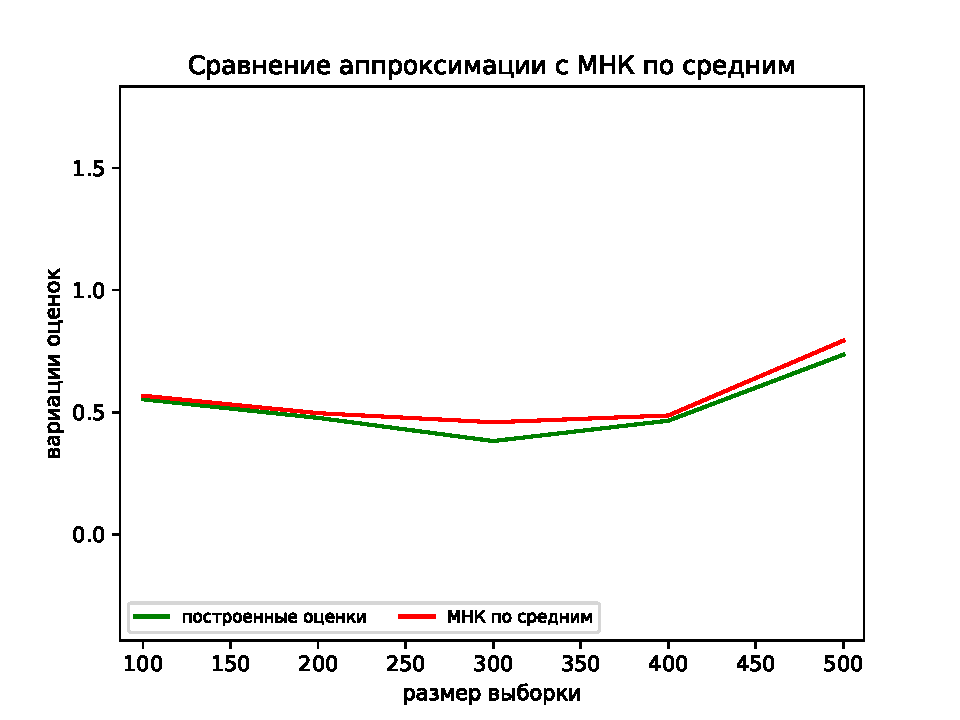
\includegraphics[width=100mm]{../images/OLS_GEM.pdf}
    \caption{Сравнение вариаций оценок\label{overflow}}
    \label{pic0}
\end{figure}
При сравнении графиков вариаций (рис.\ref{pic0}) можно сделать вывод, что ОМП дают лучший результат, 

\subsubsection{Эксперимент с полиномиальной регрессией}
Был проведен эксперимент с полиномиальной регрессией. Использовались те же параметры модели (таблица \ref{tab1}), объем выборки $N$ изменялся от 100 до 1000:
\begin{figure}[h!]
    \centering
    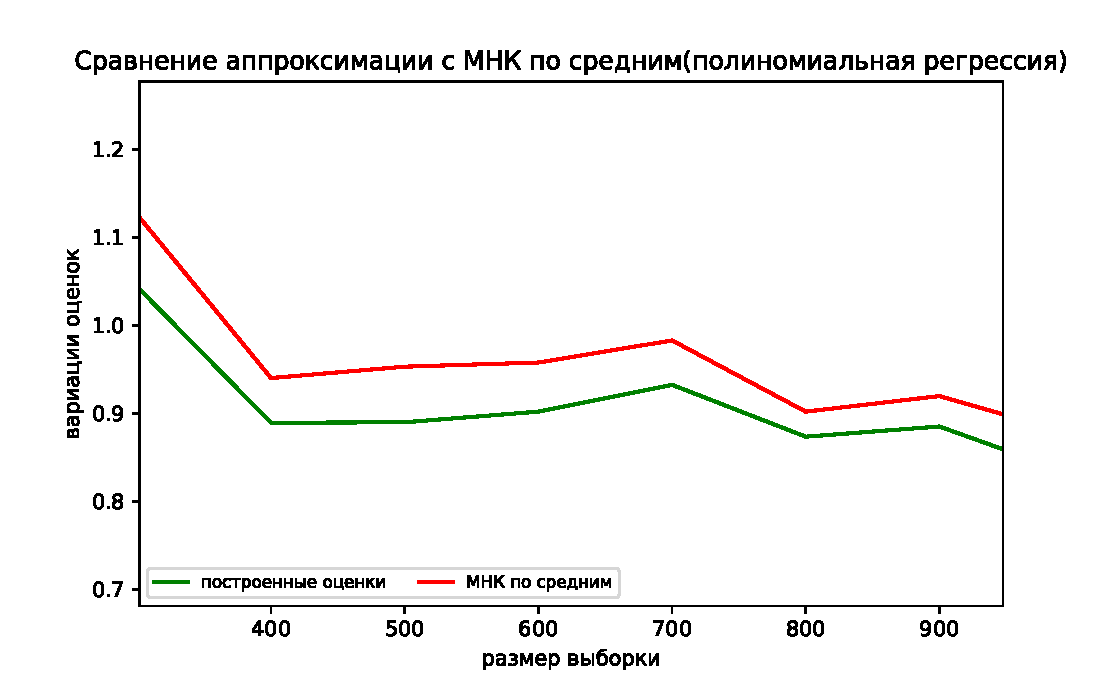
\includegraphics[width=150mm]{../images/polynomial.pdf}
    \caption{Вариации оценок в случае полиномиальной регрессии\label{overflow}}
    \label{pic3}
\end{figure}

Оба метода имели схожее поведение при изменении объема выборки, но построенные оценки максимального правдоподобия стабильно показывали лучший результат.

\newpage
\subsection{Эксперименты с изменением уровня переклассификации выборки}\label{ss3_3_1}
В ходе преддипломной практики были построены эксперименты с изменением величины K для метода $K$-ближайших соседей, используемого в переклассификации.  

Объем выборки $N$ был постоянным: $N=500$. Использовалась модель линейной регрессии. Доля выбросов была постоянна и равнялась $\widetilde{\varepsilon}=0.08$. Параметры регрессии были постоянными и равнялись $\beta=(90,4)^T$. 
Регрессоры $x_i$ были из равномерного распределения $U(-5,5)$, ошибки эспериментов $\varepsilon_i\sim \mathcal{N}(0,16)$. Величина $K$ менялась от $10$ до $40$.
\begin{center}
    \captionof{table}{Параметры модели и оценок экспериментов с переклассификацией выборки}\label{tab1}
    \begin{tabular}{|p{5cm}|p{5cm}|}
        \hline
        \multicolumn{2}{|c|}{Параметры программы} \\
        \hline
        Переменная&значение\\
        \hline
        Размер выборки $N$& 500\\
        \hline
        Доля выбросов $\widetilde{\varepsilon}$& 0.08\\
        \hline
        Параметры регрессии $\beta$& $(90,4)$\\
        \hline
        Регрессоры $x_i$ & $\sim U(-5,5)$\\
        \hline
        $\varepsilon_i$&$\sim \mathcal{N}(0,16)$\\
        \hline
        $\eta_i$&$\sim \mathcal{N}(100,100)$\\
        \hline
        Величина $K$  &от $10$ до $40$\\
        \hline
    \end{tabular},
\end{center}

\begin{figure}[h!]
    \centering
    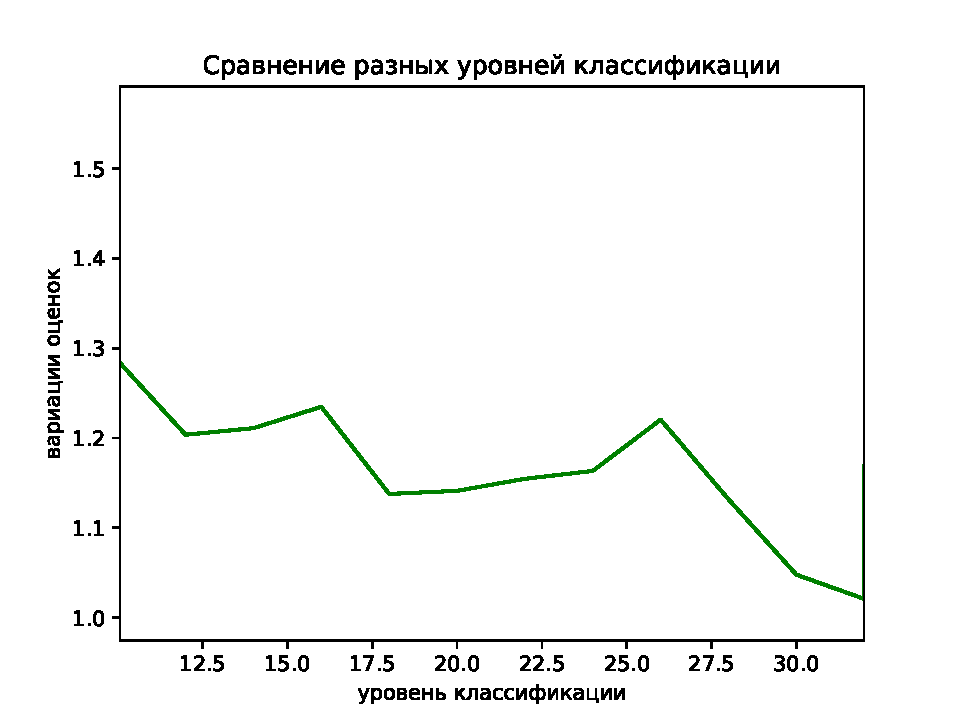
\includegraphics[width=100mm]{../images/different_recl_level.pdf}
    \caption{Зависимость вариаций от $K$ -- числа соседей, используемого в переклассификации выборки\label{overflow}}
    \label{pic1}
\end{figure}

В результате получилось, что при увеличении константы K точность оценки параметров растёт. 
\subsection{Сравнение вариаций с оценками без переклассификации}
Были проведены эксперименты для сравнения эмпирической вариации оценок максимального правдоподобия, когда использовалась вышеописанная переклассификация и когда не использовалась. При этом на каждой итерации выборка увеличивалась. 

Объем выборки $N$ изменялся от $N_1=100$ до $N_2=400$, при этом выборка дополнялась, а не генерировалась новая. Использовалась модель линейной регрессии. Доля выбросов была постоянна и равнялась $\widetilde{\varepsilon}=0.08$. Параметры регрессии были постоянными и равнялись $\beta=(90,4)^T$. 
Регрессоры $x_i$ были из равномерного распределения $U(-5,5)$, ошибки эспериментов $\varepsilon_i\sim \mathcal{N}(0,16)$. В методе, где использовалась переклассификация, величина $K$ выбиралась: $K=10$.
\vspace{3cm}
\begin{center}
    \captionof{table}{Параметры модели и оценок экспериментов}\label{tab1}
    \begin{tabular}{|p{5cm}|p{5cm}|}
        \hline
        \multicolumn{2}{|c|}{Параметры программы} \\
        \hline
        Переменная&значение\\
        \hline
        Размер выборки $N$& от 100 до 400\\
        \hline
        Доля выбросов $\widetilde{\varepsilon}$& 0.08\\
        \hline
        Параметры регрессии $\beta$& $(90,4)$\\
        \hline
        Регрессоры $x_i$ & $\sim U(-5,5)$\\
        \hline
        $\varepsilon_i$&$\sim \mathcal{N}(0,16)$\\
        \hline
        $\eta_i$&$\sim \mathcal{N}(100,100)$\\
        \hline
        В методе, с переклассификацией величина $K$& 10\\
        \hline
    \end{tabular},
\end{center}
\newpage
\begin{figure}[ht!]
    \centering
    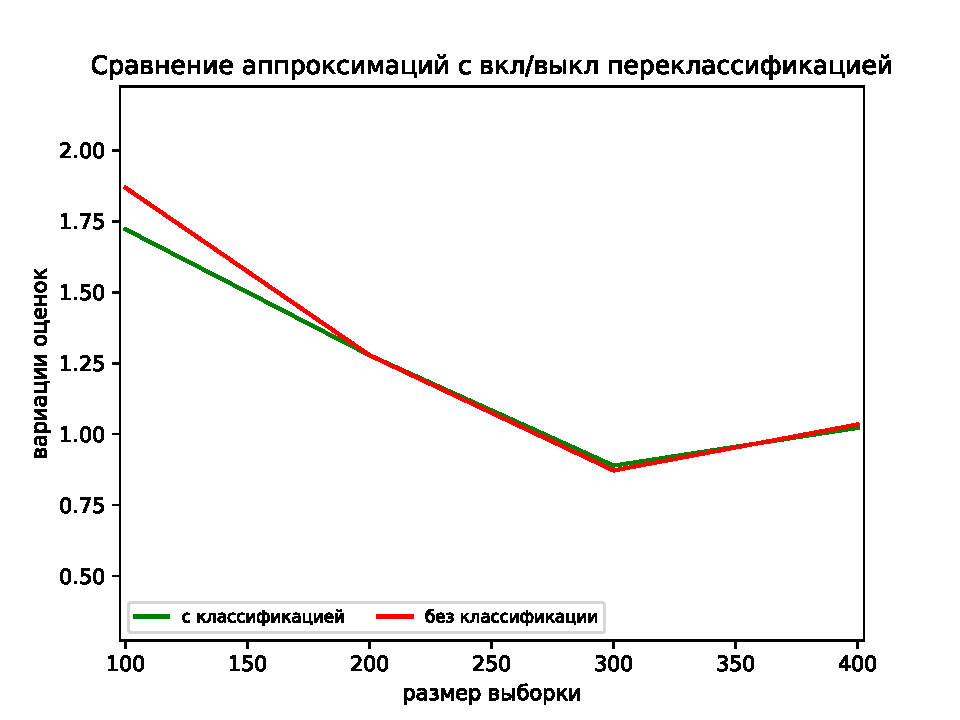
\includegraphics[width=100mm]{../images/on_off_recl.pdf}
    \caption{Сравнение вариаций оценок когда используется и не используется переклассификация\label{overflow}}
    \label{pic2}
\end{figure}

\newpage
